\def\bagrutTocEntry{\phantomsection\addcontentsline{toc}{subsection}{\texorpdfstring{سؤال $12$ امتحان $\mathrm{899271}$ سنة $2025$}{سؤال 12 امتحان 899271 سنة 2025}}\global\let\bagrutTocEntry\relax}%
\includepdf[pages=-,pagecommand={\thispagestyle{empty}\bagrutTocEntry}]{../../../bagrut_questions/oop/oop_2025_899271_12.pdf}


\ifwithsols
\begin{boxSolution}[\texorpdfstring{سؤال $12$ امتحان $\mathrm{899271}$ سنة $2025$ - فرع أ و ب (1)}{سؤال 12 امتحان 899271 سنة 2025 - فرع أ و ب (1)}]
\textbf{أ.} المخطّط الهرميّ للفئات:
\begin{center}
\begin{english}
\begin{tikzpicture}[
    classbox/.style={rectangle, draw, thick, minimum width=1.6cm, minimum height=0.65cm, font=\ttfamily\bfseries},
    inherit/.style={-{Triangle[open, length=2.6mm, width=2.6mm]}, thick, shorten >=1pt}
]
    \node[classbox] (A) at (0, 0) {A};
    \node[classbox] (B) at (0, -1.3) {B};
    \node[classbox] (C) at (-1.5, -2.6) {C};
    \node[classbox] (D) at (1.5, -2.6) {D};

    \draw[inherit] (B.north) -- (A.south);
    \draw[inherit] (C.north) -- ([xshift=-0.3cm]B.south);
    \draw[inherit] (D.north) -- ([xshift=0.3cm]B.south);
\end{tikzpicture}
\end{english}
\end{center}

\textbf{ب. (1)} الكائنات التي تكوّنت في \textenglish{Main}:
\begin{center}
\begin{english}
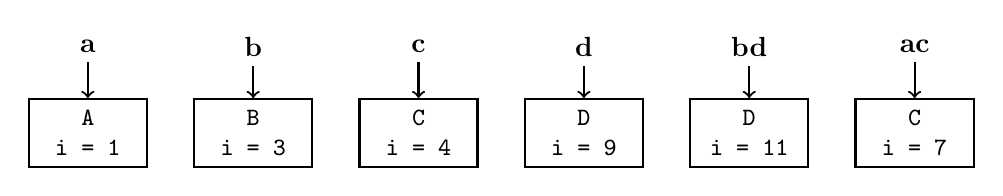
\begin{tikzpicture}[
    obj/.style={rectangle, draw, thick, align=center, font=\ttfamily\small, minimum width=1.5cm, inner sep=4pt}
]
    \node (va) at (0, 1.1) {\textbf{a}};
    \node[obj] (oa) at (0, 0) {\textbf{A}\\i = 1};
    \draw[->, thick] (va) -- (oa);

    \node (vb) at (2.1, 1.1) {\textbf{b}};
    \node[obj] (ob) at (2.1, 0) {\textbf{B}\\i = 3};
    \draw[->, thick] (vb) -- (ob);

    \node (vc) at (4.2, 1.1) {\textbf{c}};
    \node[obj] (oc) at (4.2, 0) {\textbf{C}\\i = 4};
    \draw[->, thick] (vc) -- (oc);

    \node (vd) at (6.3, 1.1) {\textbf{d}};
    \node[obj] (od) at (6.3, 0) {\textbf{D}\\i = 9};
    \draw[->, thick] (vd) -- (od);

    \node (vbd) at (8.4, 1.1) {\textbf{bd}};
    \node[obj] (obd) at (8.4, 0) {\textbf{D}\\i = 11};
    \draw[->, thick] (vbd) -- (obd);

    \node (vac) at (10.5, 1.1) {\textbf{ac}};
    \node[obj] (oac) at (10.5, 0) {\textbf{C}\\i = 7};
    \draw[->, thick] (vac) -- (oac);
\end{tikzpicture}
\end{english}
\end{center}
\end{boxSolution}

\filbreak

\begin{boxSolution}[\texorpdfstring{سؤال $12$ امتحان $\mathrm{899271}$ سنة $2025$ - فرع ب (2)}{سؤال 12 امتحان 899271 سنة 2025 - فرع ب (2)}]
\textbf{ب. (2)} مُخرجات العملية \textenglish{Main}:
\begin{boxCode}
\begin{english}
\begin{minted}{text}
// (1) c.Foo(5) -> C.Foo(int)
Foo3
True

// (2) d.Foo(a) -> B.Foo(Object)
Foo1
False

// (3) bd.Foo(b) -> B.Foo(Object)
Foo1
False

// (4) bd.Foo(b, 1) -> D.Foo(B, int) -> base.Foo(b, 20)
Foo4
Foo2
True

// (5) ((C)ac).Foo(c) -> B.Foo(Object)
Foo1
False
\end{minted}
\end{english}
\end{boxCode}
\end{boxSolution}
\fi
\filbreak
